\documentclass{article}
\usepackage{amsmath}
\usepackage{listings}
\usepackage{xcolor}
\usepackage{graphicx}
\usepackage[a4paper, total={6in, 8in}]{geometry}


\definecolor{codegreen}{rgb}{0,0.6,0}
\definecolor{codegray}{rgb}{0.5,0.5,0.5}
\definecolor{codepurple}{rgb}{0.58,0,0.82}
\definecolor{backcolour}{rgb}{0.95,0.95,0.92}

\lstdefinestyle{mystyle}{
    backgroundcolor=\color{backcolour},   
    commentstyle=\color{codegreen},
    keywordstyle=\color{magenta},
    numberstyle=\tiny\color{codegray},
    stringstyle=\color{codepurple},
    basicstyle=\ttfamily\footnotesize,
    breakatwhitespace=false,         
    breaklines=true,                 
    captionpos=b,                    
    keepspaces=true,                 
    numbers=left,                    
    numbersep=5pt,                  
    showspaces=false,                
    showstringspaces=false,
    showtabs=false,                  
    tabsize=2
}

\lstset{style=mystyle}
\setlength\parindent{0pt}


\begin{document}

\author{Eihyuk Moon, Belay Zeleke, Dongwon Kim, Akotet Yeshaw Tesema}
\title{HSS310 Final}
\maketitle

\section{Part 1}
\subsection{Problem 1}

\hspace{1em} Suppose there are \(n\) regions each of which consist of a firm and a household in the economy.
The firms' production function and the households' utility and the law of motion for capital follows the same form as in problem 7.
The total factor productivity of the firm in region \(i\) is \(z_i\) follows the AR(1) process with \(\rho_i\).
The total factor productivity is pairwise independent.
Suppose there is a goverment in the economy that taxes each firm's production and redistributes it into each region in egalitarian manner.
We can expect that the government's role will allow the value function to be the same regardless of the distribution of capital stock and the total factor productivity.
In this problem, we prove that this is in fact the case.\\ \\
The Bellman equation for this problem is written as:
\begin{align*}
    V(\mathbf{k}_t, \mathbf{z}_t) &= \max_{\mathbf{k}_{t+1}, \mathbf{n}_{t}, \mathbf{t}_{t}, \mathbf{g}_{t}} \{ \sum_{i} u_{i}\left(z_{i,t} k_{i,t}^\alpha n_{i,t}^{1-\alpha} -t_{i, t} + g_{i, t} - k_{i, t+1}, 1 - n_{i,t}\right) \\
    &+ \beta E[V(\mathbf{k}_{t+1}, \mathbf{z}_{t+1}) | I_t] \}
\end{align*}
Where \(t_1\) and \(t_2\) are the tax rates for the firms in region 1 and 2 respectively, and \(g_1\) and \(g_2\) are the transfer payments for the households in region 1 and 2 respectively.
\begin{equation}
    \text{subject to } \sum_{i} t_{i, t} = \sum_{i} g_{i, t}
\end{equation}
This equation implies that \( \sum_{i} s_{i,t} = 0 \) where \( -\mathbf{t}_{t} + \mathbf{g}_{t} = \mathbf{s}_{t}\). Which is a preservation of the total tax revenue and the total transfer payments.\\ \\
This substitution simplfies the bellman equation into:
\begin{align*}
    V(\mathbf{k}_t, \mathbf{z}_t) &= \max_{\mathbf{k}_{t+1}, \mathbf{n}_{t}, \mathbf{t}_{t}, \mathbf{g}_{t}} \{ \sum_{i} u_{i}\left(z_{i,t} k_{i,t}^\alpha n_{i,t}^{1-\alpha} + s_{i, t} - k_{i, t+1}, 1 - n_{i,t}\right) \\
    &+ \beta E[V(\mathbf{k}_{t+1}, \mathbf{z}_{t+1}) | I_t] \}
\end{align*}
The Euler equation for region \(i\) is:
\begin{equation}
    \frac{1}{c_{i, t}} =  \frac{\beta}{c_{i, t+1}} \alpha k_{i, t+1}^{\alpha - 1} n_{i, t+1}^{1-\alpha} E\left[z_{i, t+1} | I_t\right]
\end{equation}

The first order condition with respect to \(n_{i, t}\) with envelope condition is:
\begin{equation}
    \frac{\chi}{1-n_{i,t}} = \frac{1}{c_{i,t}} \cdot z_{i,t} (k_{i,t})^{\alpha}(1-\alpha)n_{i,t}^{-\alpha}
\end{equation}

The gradient with respect to \(\mathbf{s}_t\), we get:
\begin{equation}
    0 = \sum_{i} u_{i, c}\left(z_{i,t} k_{i,t}^\alpha n_{i, t}^{1-\alpha} +s_{i, t} - k_{i, t+1}, 1 - n_{i, t}\right) ds_{i, t}
\end{equation}
In other words:
\begin{equation}
    0 = \sum_{i} \frac{1}{c_{i,t}} ds_{i, t}
\end{equation}
Since \( \sum_{i} s_{i,t} = 0 \), we have \( \sum_{i} ds_{i, t} = 0 \). These equations along with \( 0 = \sum_{i} \frac{1}{c_{i,t}} ds_{i, t} \) implies
\begin{equation}
    \frac{1}{c_{i,t}} = \frac{1}{c_{j,t}} \quad \forall i, j
\end{equation}

Apply the guess-and-verify method, where \(V(\mathbf{k}_t, \mathbf{z}_t) = A + \sum_{i} B_i \log k_{i, t} + \sum_{i} C_i \log z_{i, t}\), then the Bellman equation is written as:
\begin{align*}
    A +  \sum_{i} B_i \log k_{i, t} + \sum_{i} C_i \log z_{i, t} = & \max_{\mathbf{k}_{t+1}, \mathbf{n}_{t}, \mathbf{t}_{t}, \mathbf{g}_{t}} \{ \sum_{i} u_{i}\left(z_{i,t} k_{i,t}^\alpha n_{i,t}^{1-\alpha} + s_{i, t} - k_{i, t+1}, 1 - n_{i,t}\right) \\
    & + \beta E[A + \sum_{i} B_i \log k_{i, t+1} + \sum_{i} C_i \log z_{i, t+1} | I_t] \}
\end{align*}
\begin{equation}
    B_i = \frac{\alpha}{1-\alpha\beta}
\end{equation}
\begin{equation}
    C_i = \frac{1}{(1-\rho_i)}
\end{equation}
The optimal policies are:
\begin{equation}
    n_{i,t} = \frac{{\alpha - 1}}{{\alpha \beta \chi + \alpha - \chi - 1}}
\end{equation}
\begin{equation}
    c_{i,t} = (1 -\alpha \beta) (k_{i,t}^\alpha n_{i,t}^{1 - \alpha} z_{i,t} + s_{i,t})
\end{equation}
\begin{equation}
    k_{i,t+1} = \alpha \beta (k_{i,t}^{\alpha} n_{i,t}^{1 - \alpha} z_{i,t} + s_{i,t})
\end{equation}
Since \(c_{i,t}\) is the same for all \(i\), we get:
\begin{equation}
    s_{i, t} = \frac{1}{n} \sum_{j} z_{j, t} k_{j,t}^\alpha n_{j,t}^{1-\alpha} - z_{i,t} k_{i,t}^\alpha n_{i,t}^{1 - \alpha} 
\end{equation}
In other words, the government distributes the tax revenue in consideration of different production outputs.

\subsection{Problem 2}

The spline interpolation result is as follows:\\
\begin{center}
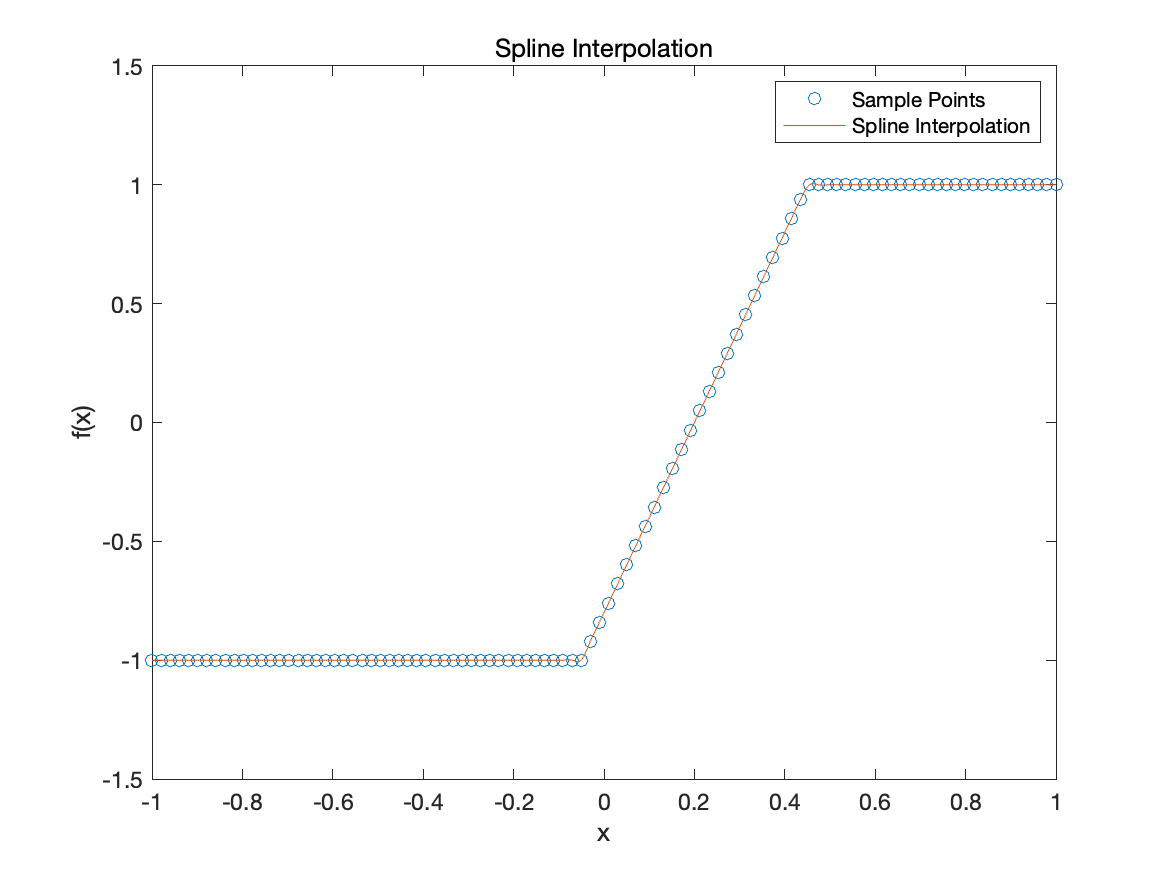
\includegraphics[scale=0.4]{spline_interpolation.png}
\end{center}
The matlab code is as follows:

\begin{lstlisting}[language=Matlab]
f = @(x) min(max(-1, 4*(x - 0.2)), 1);

x = linspace(-1, 1, 100);
y = arrayfun(f, x);
xi = linspace(-1, 1, 1000);
yi = interp1(x, y, xi, 'spline');

figure;
plot(x, y, 'o', xi, yi, '-');
legend('Sample Points', 'Spline Interpolation');
title('Spline Interpolation');
xlabel('x');
ylabel('f(x)');
print('spline_interpolation', '-dpng');

A = 1;
beta = 0.99;
delta = 0.025;
alpha = 0.36;
kmin = 0.06;
kmax = 12;
tol = 0.01;
m = 300;

k = kmin:kmin:kmax;

[V, policy] = run_bellman(k, A, beta, delta, alpha, tol, m);
[V_trivial, policy_trivial] = run_bellman(k, A, beta, 1, alpha, tol, m);

figure;
plot(k, V);
title('Value Function');
xlabel('Capital Stock k');
ylabel('Value Function V(k)');
print('value_function', '-dpng');

figure;
plot(k, policy, k, policy_trivial);
title('Policy Function');
xlabel('Capital Stock k');
ylabel('Optimal k''');
legend('delta = 0.025', 'delta = 1');
print('policy_function', '-dpng');

function [V, policy] = run_bellman(k, A, beta, delta, alpha, tol, m)
n = length(k);
V = zeros(1, n);

for iter = 1:m
    Vnew = zeros(1, n);
    for i = 1:n
        obj = @(j) (log(A*k(i)^alpha + (1-delta)*k(i) - k(j)) + beta*V(j));
        
        jmax = find(k <= A*k(i)^alpha + (1-delta)*k(i), 1, 'last');
        [val, ip] = max(arrayfun(obj, 1:jmax));
        
        if A*k(i)^alpha + (1-delta)*k(i) - k(ip) <= 0
            val = -Inf;
        end
        
        Vnew(i) = val;
    end
    
    if max(abs(V - Vnew)) < tol
        break;
    end
    V = Vnew;
end

policy = zeros(1, length(k));
for i = 1:n
    obj = @(kp) -(log(A*k(i)^alpha + (1-delta)*k(i) - kp) + beta*interp1(k, V, kp, 'spline'));
    [kp_opt, ~] = fminbnd(obj, 0, A*k(i)^alpha + (1-delta)*k(i));
    policy(i) = kp_opt;
end
end
\end{lstlisting}

The results for the code is as follows:\\
\begin{center}
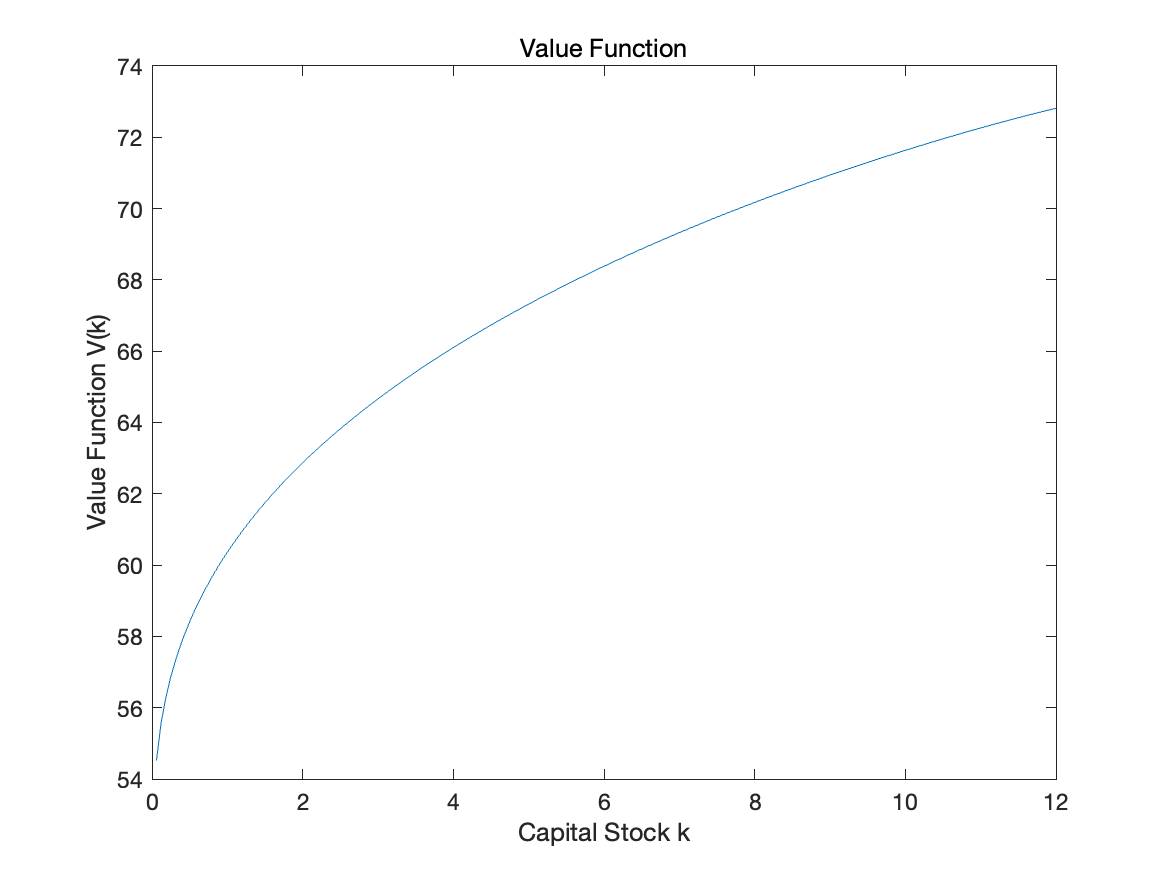
\includegraphics[scale=0.4]{value_function.png}\\
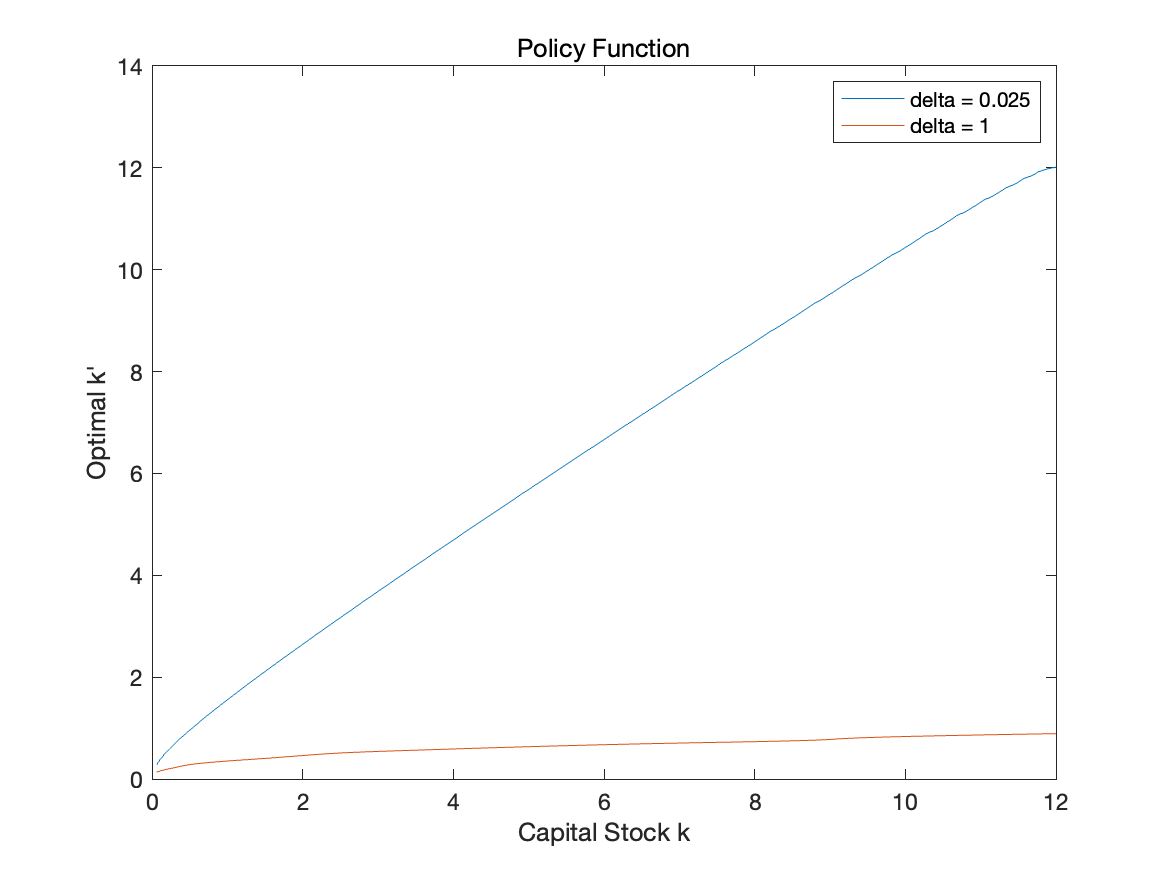
\includegraphics[scale=0.4]{policy_function.png}
\end{center}


\section{Part 2}

\subsection{}

\[
\max_{\{k_{t+1}, c_t, n_t, y_t, i_t\}} E^P \left( \sum_{t=0}^{\infty} \beta^{t} u(c_t, 1 - n_t) \,|\, I_0 \right) \text{subject to } y_t = i_t + c_t,\\
\]
\[
k_{t+1} = (1 - \delta) k_t + i_t,\\
\]
\[
y_t = z_t k_t^\alpha n_t^{1 - \alpha},\\
\]
\[
0 \leq n_t \leq 1,\\
\]
\[
k_0, z_0: \text{ given},\\
\]
\[
\{ z_t \}: \text{a random process},\\
\]

\[
P \equiv \text{\{subjective probability distribution at the individual level or} \\
\]
\[
\text{objective distribution in equilibrium (rational expectations)\}}.
\]

\subsection{}
For any function $g(\cdot, \cdot) \in S_{K \times Z}$, any $I_{t+1}$-measurable random variable $z_{t+1}$ distributed on $Z \equiv [z_{\text{min}}, z_{\text{max}}]$, and any realized value of $z_t$, there exists a continuous and bounded function $h(\cdot, \cdot) \in S_{K \times Z}$ such that for all $t \geq 0$, 
\begin{equation}
    E[g(k_{t+1},z_{t+1})|I_t] = h(k_{t+1}, z_t) \in S_{K \times Z}
\end{equation}

\subsection{}
The transformation $T(g(k_{t+1},z_{t+1}))$ is given by:
\begin{equation}
    T(g(k_{t+1},z_{t+1})) = \max_{k_{t+1},n_t} u\left(z_t k_t^\alpha n_t^{1-\alpha} + (1-\delta) k_t - k_{t+1}, 1 - n_t\right) + \beta E[g(k_{t+1},z_{t+1})|I_t]
\end{equation}
By applying the Feller property, the transformation can be rewritten as:
\begin{equation}
    T(g(k_{t+1},z_{t+1})) = \max_{k_{t+1},n_t} u\left(z_t k_t^\alpha n_t^{1-\alpha} + (1-\delta) k_t - k_{t+1}, 1 - n_t\right) + \beta h(k_{t+1},z_{t})
\end{equation}
Let $(k^*_{t+1},n^*_t) \equiv F(k_t)$ be the optimal choice and set
\begin{equation}
    u\left(z_t k_t^\alpha (n^*_t)^{1-\alpha} + (1-\delta) k_t - k^*_{t+1}, 1 - n^*_t\right) + \beta h(k^*_{t+1},z_{t})
\end{equation}
as the maximum achievable value given the parameter $k_t$. Since $h(\cdot, \cdot) \in S_{K \times Z}$, $h$ is continuous and bounded. $u$ is trivially continuous and bounded.

Then, by the maximum theorem, the expression
\begin{equation}
    u\left(z_t k_t^\alpha (n^*_t)^{1-\alpha} + (1-\delta) k_t - k^*_{t+1}, 1 - n^*_t\right) + \beta h(k^*_{t+1},z_{t})
\end{equation}
is continuous with respect to the parameter $k_t$. In other words, the Bellman operator
\begin{equation}
    T(g(k_{t+1},z_{t+1})) = \max_{k_{t+1},n_t} u\left(z_t k_t^\alpha n_t^{1-\alpha} + (1-\delta) k_t - k_{t+1}, 1 - n_t\right) + \beta E[g(k_{t+1},z_{t+1})|I_t]
\end{equation}
is a well-defined mapping from $S_{K \times Z}$ onto $S_{K \times Z}$.


\subsection{}
We can briefly expand Blackwell's Sufficiency Theorem for the two-dimensional case. For all functions $f, g \in S_{K \times Z}$, if $f$ and $g$ satisfy
\begin{equation}
    \forall t \in K \times Z, \ f(t) \leq g(t),
\end{equation}
then
\begin{equation}
    \forall t \in K \times Z, \ (Tf)(k) \leq (Tg)(g).
\end{equation}

Furthermore, for any function $f \in S_{K \times Z}$ and any non-negative scalar $a \geq 0$, we have

\begin{align}
    T((g+a)(k_{t+1},z_{t+1})) &= \max_{k_{t+1},n_t} u\left(z_t k_t^\alpha n_t^{1-\alpha} + (1-\delta) k_t - k_{t+1}, 1 - n_t\right) \\
    &\quad + \beta E[(g+a)(k_{t+1},z_{t+1})|I_t] \\
    &= \max_{k_{t+1},n_t} u\left(z_t k_t^\alpha n_t^{1-\alpha} + (1-\delta) k_t - k_{t+1}, 1 - n_t\right) \\
    &\quad + \beta E[g(k_{t+1},z_{t+1})|I_t] + \beta \cdot a \\
    &= T(g(k_{t+1},z_{t+1})) + \beta \cdot a,
\end{align}

where $0 < \beta < 1$. \\

For all $t \in K \times Z$, we have
\begin{equation}
    |f(t) - g(t)| \leq ||f - g||
\end{equation}
Therefore,
\begin{align*}
    \forall t \in K \times Z, \ &f(t) \leq g(t) + ||f - g|| \\
    \text{or} \ &g(t) \leq f(t) + ||f - g||
\end{align*}
This implies that
\begin{align}
    Tf &\leq T(g + ||f - g||) \leq Tg + \beta ||f - g|| \\
    \text{or} \ &Tg \leq T(f + ||f - g||) \leq Tf + \beta ||f - g||
\end{align}
Thus, we conclude that
\begin{equation}
    ||Tf - Tg|| \leq \beta ||f - g||
\end{equation}\\
and $T$ is a contraction mapping with modulus $\beta$ of $S_{K \times Z}$ onto $S_{K \times Z}$.


\subsection{}
The Bellman equation for this problem is written as:
\[ V(k_t, z_t) = \max_{k_{t+1}, n_t} \left\{ u\left(z_t k_t^\alpha n_t^{1-\alpha} + (1-\delta) k_t - k_{t+1}, 1 - n_t\right) + \beta E[V(k_{t+1}, z_{t+1}) | I_t] \right\} \]

\[\text{subject to } k_t, z_t \text{ given}\]
\[\text{and } I_t \text{ given} \]

From problem 4, we know that the Bellman operator $T$ is a contraction mapping of $S_{K \times Z}$ onto $S_{K \times Z}$ with modulus $\beta$. 
Therefore, the Bellman equation has a unique solution $V^*$ in $S_{K \times Z}$. 

\subsection{}

The first-order condition and differentiation under conditional expectation sign dictates:
\begin{equation}
    \partial{k_{t+1}}:  -u_c\left(c_t, 1 - n_t\right) + \beta E[V_k(k_{t+1}, z_{t+1}) | I_t] = 0
\end{equation}
\begin{equation}
    \partial{n_t}: -u_n\left(c_t, 1 - n_t\right) + \beta E[V_k(k_{t+1}, z_{t+1}) z_t (k_t)^{\alpha}(1-\alpha)n_t^{-\alpha}| I_t] = 0
\end{equation}
where $u_c$ is the marginal utility of consumption, and $V_k$ is the partial derivative of $V$ with respect to $k$. \\

The envelope condition dictates:
\begin{equation}
    \partial{k_t}: V_k(k_t, z_t) = u_c\left(c_t, 1 - n_t\right) \cdot \left(z_t \alpha k_t^{\alpha - 1} n_t^{1-\alpha} + 1 - \delta\right)
\end{equation}

Combining the above two equations, we have:
\begin{equation}
    -u_c\left(c_t, 1 - n_t\right) + \beta E[u_c\left(c_{t+1}, 1 - n_{t+1}\right) \cdot \left(z_{t+1} \alpha k_{t+1}^{\alpha - 1} n_{t+1}^{1-\alpha} + 1 - \delta\right) | I_t] = 0
\end{equation}
\begin{equation}
    \frac{1}{c_t} = \beta E\left[\frac{1}{c_{t+1}} \cdot \left(z_{t+1} \alpha k_{t+1}^{\alpha - 1} n_{t+1}^{1-\alpha} + 1 - \delta\right) | I_t\right]
\end{equation}
\begin{equation}
    \frac{1}{c_t} =  \frac{\beta}{c_{t+1}} \left( \alpha k_{t+1}^{\alpha - 1} n_{t+1}^{1-\alpha} E\left[z_{t+1} | I_t\right] + \left(1 - \delta\right) \right)
\end{equation}
From (19), we get:
\begin{equation}
    \frac{\chi}{1-n_t} = \beta E\left[\frac{1}{c_{t+1}} \cdot \left(z_{t+1} \alpha k_{t+1}^{\alpha - 1} n_{t+1}^{1-\alpha} + 1 - \delta\right)  \cdot z_t (k_t)^{\alpha}(1-\alpha)n_t^{-\alpha} | I_t\right]
\end{equation}
\begin{equation}
    \frac{\chi}{1-n_t} = \frac{1}{c_t} \cdot z_t (k_t)^{\alpha}(1-\alpha)n_t^{-\alpha}
\end{equation}
For capital accumulation, we have:
\begin{equation}
    k_{t+1} = z_t k_t^\alpha n_t^{1-\alpha} + (1-\delta) k_t - c_t
\end{equation}

\subsection{}

Suppose \(V(k_t, z_t) = A + B \log k_t + C \log z_t\), and for \(\delta = 1.0\), we have:
\[\frac{1}{c_t} =  \frac{\beta}{c_{t+1}} \alpha k_{t+1}^{\alpha - 1} n_{t+1}^{1-\alpha} E\left[z_{t+1} | I_t\right] \]
\[k_{t+1} = z_t k_t^\alpha n_t^{1-\alpha} - c_t\]
Bellman equation is written as:\\
\begin{align*}
    A +  B \log k_t + C \log z_t = & \max_{k_{t+1}, n_t} \{ \log\left(z_t k_t^\alpha n_t^{1-\alpha} - k_{t+1}\right)\left( 1 - n_t\right)^\chi \\
    & + \beta E[A + B \log k_{t+1} + C \log z_{t+1} | I_t] \}
\end{align*}

The first order condition with respect to \(k_{t+1}\) is:
\begin{equation}
   0 = \frac{{B \cdot \beta}}{{k_{t1}}} - \frac{1}{{k_t^{\alpha} \cdot n_t^{(1 - \alpha)} \cdot z_t - k_{t1}}}
\end{equation}

The first order condition with respect to \(n_t\) is:
\begin{equation}
    0 = -\frac{{\chi}}{{1 - n_t}} + \frac{{k_t^{\alpha} \cdot n_t^{(1 - \alpha)} \cdot z_t \cdot (1 - \alpha)}}{{n_t \cdot (k_t^{\alpha} \cdot n_t^{(1 - \alpha)} \cdot z_t - k_{t1})}}
\end{equation}

Suppose the optimal choice is \(k^*_{t+1}\) and \(n^*_t\), then we have:

\begin{equation}
    k^*_{t+1} = \frac{\beta B}{1 + \beta B} z_t k_t^\alpha n_t^{1-\alpha}
\end{equation}

\begin{equation}
    n^*_t = \frac{{\alpha - 1}}{{\alpha \beta \chi + \alpha - \chi - 1}}
\end{equation}

\begin{align*}
    A +  B \log k_t + C \log z_t = & \log\left(z_t k_t^\alpha n_t^{* 1-\alpha} - k^*_{t+1}\right) + \chi \log\left( 1 - n^*_t\right) \\
    & + \beta A + \beta B \log k^*_{t+1} + \beta C \rho \log z_t
\end{align*}

Using \(k^*_{t+1}\) we have:
\begin{align*}
    A +  B \log k_t + C \log z_t &= \beta ( A + B \log ( \frac{B \beta k_t^\alpha n_t^{* 1 - \alpha} z_t}{B \beta + 1} ) \\
    &+ C \rho \log(z_t) ) + \chi \log\left( 1 - n^*_t\right) + \log ( k_t^\alpha n_t^{1 - \alpha} z_t - \frac{B \beta k_t^\alpha n_t^{1 - \alpha} z_t}{B \beta + 1} )
\end{align*}

Then, the coefficients are:\\
\begin{equation}
    A = \frac{(1-\alpha)\log(n^*_t) + (1 - \alpha\beta)\chi\log(1 - n^*_t) + \alpha\beta\log(\alpha\beta) +(1- \alpha\beta)\log(1-\alpha\beta)}{(1 - \alpha\beta)(1 - \beta)}
\end{equation}

\begin{equation}
    B = \frac{\alpha}{1-\alpha\beta}
\end{equation}

\begin{equation}
    C = \frac{1}{(1-\alpha\beta)(1-\rho)}
\end{equation}

The optimal policy functions are:\\
\begin{equation}
    n_t = \frac{{\alpha - 1}}{{\alpha \beta \chi + \alpha - \chi - 1}}
\end{equation}

\begin{equation}
    c_t = (1 -\alpha \beta) k_t^\alpha n_t^{1 - \alpha} z_t
\end{equation}

\begin{equation}
    k_{t+1} = \alpha \beta k_{t}^{\alpha} n_{t}^{1 - \alpha} z_{t}
\end{equation}

\subsection{}
Bellman equation is written as:\\
\begin{equation}
    V(k_t, z_t) = \max_{k_{t+1}, n_t} \left\{ u\left(z_t k_t^\alpha n_t^{1-\alpha}-i_t, 1 - n_t\right) + \beta E[V(k_{t+1}, z_{t+1}) | I_t] \right\}
\end{equation}
For simplification, we maximize w.r.t. \(i_t\), since determining \(i_t\) is equivalent to determining \(k_{t+1}\). \\ \\
Suppose \(V(k_t, z_t) = A + B \log k_t + C \log z_t\), then we have:
\begin{align*}
    A +  B \log k_t + C \log z_t = & \max_{i_{t}, n_t} \{ \log\left(z_t k_t^\alpha n_t^{1-\alpha}-i_t\right) + \chi\log\left( 1 - n_t\right) \\
    &  + \beta A + \beta B \log (k_{t})^{1-\delta}(i_t)^\delta + \beta \rho C \log z_{t} \}
\end{align*}
First order condition with respect to \(i_t\):\\
\begin{equation}
    0 = \frac{{B \cdot \beta \cdot \delta}}{i_t} - \frac{1}{{-i_t + k_t^{\alpha} \cdot n_t^{(1 - \alpha)} \cdot z_t}}
\end{equation}\\
First order condition with respect to \(n_t\):\\
\begin{equation}
    0 = -\frac{{\chi}}{{1 - n_t}} + \frac{{k_t^{\alpha} \cdot n_t^{(1 - \alpha)} \cdot z_t \cdot (1 - \alpha)}}{{n_t \cdot (-i_t + k_t^{\alpha} \cdot n_t^{(1 - \alpha)} \cdot z_t)}}
\end{equation}\\
After solving the above two equations, we have:\\
\begin{equation}
    B = \frac{\alpha}{1-\beta(1-\delta)-\alpha\beta\delta}
\end{equation}
\begin{equation}
    C = \frac{1}{(1-\rho\beta)}
\end{equation}

\begin{equation}
    i_t^* = \frac{B\beta\delta k_t^\alpha n_t^{1 - \alpha}z_t}{B\beta\delta + 1}
\end{equation}

\begin{equation}
    n_t^* = \frac{-B\alpha\beta\delta + B\beta\delta - \alpha + 1}{-B\alpha\beta\delta + B\beta\delta - \alpha + \chi + 1}
\end{equation}\\

Therefore, for control variables, we have:\\
\begin{equation}
    c_t = \frac{k_t^\alpha n_t^{1-\alpha} z_t (-\alpha\beta\delta + \beta\delta - \beta + 1)}{\beta\delta - \beta + 1}
\end{equation}

\begin{equation}
    n_t = \frac{\alpha\beta\delta - \alpha\beta + \alpha - \beta\delta + \beta - 1}{\alpha\beta\chi\delta + \alpha\beta\delta - \alpha\beta + \alpha - \beta\chi\delta + \beta\chi - \beta\delta + \beta - \chi - 1}
\end{equation}\\

For state variables, we have:\\
\begin{equation}
    k_{t+1} = k_t^{1-\delta} \left(\frac{\alpha\beta\delta k_t^\alpha n_t^{1-\alpha} z_t}{\beta\delta - \beta + 1}\right)^\delta
\end{equation}


\hspace{1em} The law of motion for capital can be written as \(k_{t+1} = k_t(\frac{i_t}{k_t})^{1-\delta}\) and a few observations can be made from this.
First, the investment should be always nonzero, otherwise the capital stock will be zero in the next period.
This is similar to the Brock-Mirman model with \(\delta = 1\), where investment should be positive for capital accumulation.
However, this is not true for the Brock-Mirman model with \(0 < \delta < 1\), where the capital stock does not immediately become zero in the next period even if the investment is zero.
Second, unlike the Brock-Mirman model, the investment is not additive to the capital stock, but rather multiplicative and scaled.
The capital in the next time step exhibits constant returns to scale in capital and investment.
This implies that the investment should be larger than the current capital stock \(k_t\), otherwise the capital stock begins to shrink.
The Brock-Mirman model differs in that the investment should larger than \(\delta k_t\) for the capital stock to grow.
Third, the concavity of this investment-capital ratio implies diminishing marginal return of investment.
This is also what differs from the Brock-Mirman model, where marginal return of investment is constant.
This relation is referred to as \textit{the capital adjustment cost} in our survey of the literature.\\

The business cycle implications are as follows:
\begin{equation}
    \mathrm{Var}[\log i_t^*] = \mathrm{Var}[\log c_t^*] = \mathrm{Var}[\log y_t^*]
\end{equation}
This result is the same as the Brock-Mirman model with \(\delta = 1\).

\subsection{}
The Bellman equation for this problem is written as:
\begin{equation}
    V(k_t, z_t) = \max_{k_{t+1}, n_t} \left\{ \log\left(z_t k_t^\alpha n_t^{1-\alpha}-i_t-\chi (n_t)^{1+\omega}\right) + \beta E[V(k_{t+1}, z_{t+1}) | I_t] \right\}
\end{equation}
For simplification, we maximize w.r.t. \(i_t\), since determining \(i_t\) is equivalent to determining \(k_{t+1}\). \\ \\
Suppose \(V(k_t, z_t) = A + B \log k_t + C \log z_t\), then we have:
\begin{align*}
    A +  B \log k_t + C \log z_t = & \max_{i_{t}, n_t} \{ \log\left(z_t k_t^\alpha n_t^{1-\alpha}-i_t-\chi (n_t)^{1+\omega}\right) \\
    &  + \beta A + \beta B (1-\delta) \log (k_{t}) + \beta B \delta \log(i_t) + \beta \rho C \log z_{t} \}
\end{align*}
First order condition with respect to \(i_t\):\\
\begin{equation}
    i_t^* = \frac{{B \cdot \beta \cdot \delta \cdot (-\chi \cdot n_t^{(\omega + 1)} + k_t^{\alpha} \cdot n_t^{(1 - \alpha)} \cdot z_t)}}{{B \cdot \beta \cdot \delta + 1}}
\end{equation}
First order condition with respect to \(n_t\):\\
\begin{equation}
    n_t^* = \left(\frac{1-\alpha}{\chi (1+\omega)}\right)^{\frac{1}{\omega + \alpha}} \left(k_t^\alpha z_t\right)^{\frac{1}{\omega + \alpha}}
\end{equation}
\begin{equation}
    y_t^* = \left(\frac{1-\alpha}{\chi (1+\omega)}\right)^{\frac{1-\alpha}{\alpha + \omega}} \left(k_t^\alpha z_t\right)^{\frac{\omega + 1}{\omega + \alpha}}
\end{equation}

Suppose \(\overline{a} = \left(\frac{1-\alpha}{\chi (1+\omega)}\right)^{\frac{1}{\alpha + \omega}}\), then we have:
\begin{equation}
\log(y_t^* -\chi \cdot n_t^{(\omega + 1)}) = \log\left(\overline{a}^{1-\alpha} - \chi \overline{a}^{1+\omega}\right)+ \frac{\alpha(\omega + 1)}{\omega + \alpha} \log (k_{t}) + \frac{\omega + 1}{\omega + \alpha} \log(z_t)
\end{equation}


\begin{align*}
    A +  B \log k_t + C \log z_t = & -\log\left(1+B\beta\delta\right) + \log\left(\overline{a}^{1-\alpha} - \chi \overline{a}^{1+\omega}\right) \\
    & + \frac{\alpha(\omega + 1)}{\omega + \alpha} \log (k_{t}) + \frac{\omega + 1}{\omega + \alpha} \log(z_t) \\
    &  + \beta A + \beta B (1-\delta) \log (k_{t}) + \beta B \delta \log(i_t) + \beta \rho C \log z_{t}
\end{align*}


\begin{align*}
    A +  B \log k_t + C \log z_t = &\left(B\beta\delta\right) \log\left(B\beta\delta\right)-\left(1+B\beta\delta\right) \log\left(1+B\beta\delta\right) + \beta A\\
    &\left(1+B\beta\delta\right)\log\left(\overline{a}^{1-\alpha} - \chi \overline{a}^{1+\omega}\right)+ \left(1+B\beta\delta\right)\frac{\alpha(\omega + 1)}{\omega + \alpha} \log (k_{t}) + \left(1+B\beta\delta\right)\frac{\omega + 1}{\omega + \alpha} \log(z_t) \\
    &\beta B (1-\delta) \log (k_{t}) + \beta \rho C \log z_{t}
\end{align*}

\begin{equation} 
    B = \frac{\alpha(-\omega - 1)}{\alpha\beta\delta\omega + \alpha\beta - \alpha - \beta\delta\omega + \beta\omega - \omega} 
\end{equation}

\begin{equation}
   C = \frac{{(\omega + 1)  (\alpha  \beta  \delta - \alpha  \beta + \alpha + \beta  \delta  \omega - \beta  \omega + \omega)}}{{(\alpha  \beta  \rho - \alpha + \beta  \omega  \rho - \omega)  (\alpha  \beta  \delta  \omega + \alpha  \beta - \alpha - \beta  \delta  \omega + \beta  \omega - \omega)}}
\end{equation}

\begin{equation}
    i_t^* = \frac{{\alpha  \beta  \delta  (\omega + 1)  (k_t^{\alpha}  n_t^{(1 - \alpha)}  z_t - \chi  n_t^{(\omega + 1)})}}{{\alpha  \beta  \delta  - \alpha  \beta + \alpha + \beta  \delta  \omega - \beta  \omega + \omega}}
\end{equation}

The optimal household polices are:
\begin{equation}
    n_t = \left(\frac{1-\alpha}{\chi (1+\omega)}\right)^{\frac{1}{\omega + \alpha}} \left(k_t^\alpha z_t\right)^{\frac{1}{\omega + \alpha}}
\end{equation}

\begin{equation}
    k_{t+1} = k_t^{\delta} \left(\frac{{\alpha  \beta  \delta  (\omega + 1)  (k_t^{\alpha}  n_t^{(1 - \alpha)}  z_t - \chi  n_t^{(\omega + 1)})}}{{\alpha  \beta  \delta  - \alpha  \beta + \alpha + \beta  \delta  \omega - \beta  \omega + \omega}}\right)^{1-\delta}
\end{equation}

\begin{equation}
    c_t = y_t - i_t
\end{equation}

\end{document}